\documentclass[tikz,border=4pt]{standalone}
\usepackage{amsmath,amssymb}
% Grupo Nostradamus - lenguaje visual TikZ
\definecolor{nostranavy}{HTML}{061426}
\definecolor{nostrateal}{HTML}{078C95}
\definecolor{nostracyan}{HTML}{65DCE5}
\definecolor{nostragold}{HTML}{F5C542}
\newcommand{\sen}{\operatorname{sen}}

\begin{document}
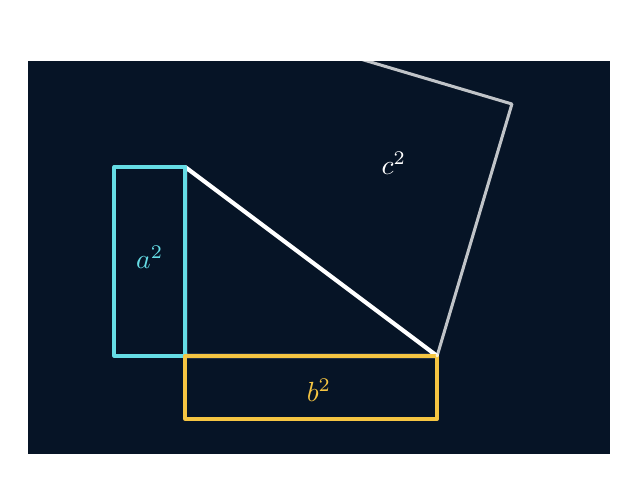
\begin{tikzpicture}[line cap=round,line join=round]
\fill[nostranavy] (-3.7,-2.5) rectangle (3.7,2.5);
\coordinate (A) at (-1.7,-1.25);\coordinate (B) at (1.5,-1.25);\coordinate (C) at (-1.7,1.15);
\draw[white,line width=1.5pt] (A)--(B)--(C)--cycle;
\draw[nostracyan,line width=1.3pt] (-1.7,-1.25) rectangle (-2.6,1.15);
\draw[nostragold,line width=1.3pt] (-1.7,-1.25) rectangle (1.5,-2.05);
\draw[white,opacity=.75,line width=1.1pt] (1.5,-1.25)--(2.45,1.95)--(-.75,2.90);
\node[nostracyan,font=\bfseries] at (-2.15,0) {$a^2$};
\node[nostragold,font=\bfseries] at (0,-1.68) {$b^2$};
\node[white,font=\bfseries] at (.95,1.20) {$c^2$};
\end{tikzpicture}
\end{document}
